\chapter[Experimentos e Resultados]{Experimentos e Resultados}
\label{cap:experimentos}

Neste capítulo são descritos os experimentos conduzidos no desenvolvimento do
RECLin-PT, com foco na classe \texttt{negation\_of}, bem como os resultados obtidos
até o momento, todos no conjunto de desenvolvimento. Cada experimento responde a uma
decisão de configuração do modelo: a comparação entre \emph{encoders}, à escolha do
\emph{encoder}, e a comparação entre estratégias, à escolha da estratégia. Este
capítulo reporta o que foi observado; o que esses resultados implicam para o
RECLin-PT é discutido no Capítulo~\ref{cap:discussao}. A \autoref{fig:ciclo} apresenta
o ciclo de desenvolvimento e o estado atual de cada etapa. A preparação dos dados e a
geração de pares candidatos estão concluídas. O \emph{fine-tuning} foi realizado
apenas para parte das combinações de \emph{encoder} e estratégia, e a seleção de
épocas e de limiares no DEV foi feita para todas as execuções existentes. A
comparação é parcial: as estratégias foram comparadas com o BioBERTpt-all, e os
\emph{encoders}, apenas na estratégia baseline, de forma descritiva e no DEV. O
congelamento da configuração, a avaliação única no conjunto de teste e a seleção da
configuração final do RECLin-PT permanecem pendentes. A seta de retorno indica que
novos \emph{encoders} ou estratégias voltam à etapa de \emph{fine-tuning} antes de
entrar na comparação.

% Ciclo de desenvolvimento do RECLin-PT, com o estado de cada etapa conferido
% nos artefatos (branch resultados-colab, commit bb9457f) e no protocolo.
\begin{figure}[htbp]
  \centering
  \caption{Ciclo de desenvolvimento do RECLin-PT e estado atual de cada etapa.}
  \label{fig:ciclo}
  \begin{tikzpicture}[
      font=\sffamily\footnotesize,
      etapa/.style={rounded corners=3pt, minimum height=1.25cm, text width=3.0cm, align=center, inner sep=3pt},
      concluida/.style={etapa, draw=black!80, fill=black!20, line width=0.8pt},
      parcial/.style={etapa, draw=black!80, line width=0.8pt, fill=white, pattern=north east lines, pattern color=black!25},
      pendente/.style={etapa, draw=black!60, dashed, line width=0.8pt, fill=white},
      seta/.style={-{Stealth[length=2.2mm]}, line width=0.8pt},
      estado/.style={font=\sffamily\scriptsize\itshape, text=black!70, below=1.5pt}
    ]
    % linha 1 (da esquerda para a direita)
    \node[concluida] (e1) at (0,0)    {\textbf{1.} Preparação\\ dos dados};
    \node[concluida] (e2) at (3.75,0) {\textbf{2.} Geração de\\ pares candidatos};
    \node[parcial]   (e3) at (7.5,0)  {\textbf{3.} \emph{Fine-tuning}\\ (\emph{encoder} $\times$ estratégia)};
    \node[concluida] (e4) at (11.25,0){\textbf{4.} Seleção de épocas\\ e limiares no DEV};
    % linha 2 (da direita para a esquerda)
    \node[parcial]   (e5) at (11.25,-3.4) {\textbf{5.} Comparação de\\ estratégias e \emph{encoders}};
    \node[pendente]  (e6) at (7.5,-3.4)   {\textbf{6.} Congelamento\\ da configuração};
    \node[pendente]  (e7) at (3.75,-3.4)  {\textbf{7.} Avaliação única\\ no TEST};
    \node[pendente]  (e8) at (0,-3.4)     {\textbf{8.} Seleção do\\ modelo final};
    \draw[seta] (e1) -- (e2);
    \draw[seta] (e2) -- (e3);
    \draw[seta] (e3) -- (e4);
    \draw[seta] (e4.south) -- (e5.north);
    \draw[seta] (e5) -- (e6);
    \draw[seta] (e6) -- (e7);
    \draw[seta] (e7) -- (e8);
    % retorno 5 -> 3
    \draw[seta, dashed] (9.95,-2.775) -- (9.95,-1.7) -- (8.35,-1.7) -- (8.35,-0.625);
    \node[font=\sffamily\scriptsize, anchor=north east] at (9.85,-1.78) {novos \emph{encoders} ou estratégias};
    % estados
    \node[estado] at (e1.south) {concluída};
    \node[estado] at (e2.south) {concluída};
    \node[estado, xshift=-6mm] at (e3.south) {parcial$^{a}$};
    \node[estado, xshift=-8mm] at (e4.south) {concluída$^{b}$};
    \node[estado, xshift=-8mm] at (e5.south) {parcial$^{c}$};
    \node[estado] at (e6.south) {pendente};
    \node[estado] at (e7.south) {pendente};
    \node[estado] at (e8.south) {pendente};
    % legenda
    \begin{scope}[shift={(3.9,-4.95)}, font=\sffamily\scriptsize]
      \node[draw=black!80, fill=black!20, minimum width=5mm, minimum height=3.2mm, rounded corners=1pt] (l1) at (0,0) {};
      \node[right=1mm of l1] (t1) {concluída};
      \node[draw=black!80, fill=white, pattern=north east lines, pattern color=black!25, minimum width=5mm, minimum height=3.2mm, rounded corners=1pt, right=6mm of t1] (l2) {};
      \node[right=1mm of l2] (t2) {parcial};
      \node[draw=black!60, dashed, fill=white, minimum width=5mm, minimum height=3.2mm, rounded corners=1pt, right=6mm of t2] (l3) {};
      \node[right=1mm of l3] {pendente};
    \end{scope}
  \end{tikzpicture}\\[4pt]
  {\footnotesize $^{a}$ O BioBERTpt-all foi ajustado em todas as estratégias treinadas; o BERTimbau-base, apenas no baseline; o BioBERTpt-clin e o \emph{fine-tuning} restrito não têm execução. $^{b}$ Para as execuções existentes e verificadas. $^{c}$ Estratégias comparadas com o BioBERTpt-all; \emph{encoders}, apenas na estratégia baseline; comparações descritivas no DEV.}\\[2pt]
  {\footnotesize Fonte: elaborado pelo autor.}
\end{figure}


Todos os números são do conjunto de desenvolvimento (DEV), com semente $42$, sobre os
$19\,064$ pares candidatos das partições congeladas (Seção~\ref{sec:candidatos}). O
DEV é o mesmo conjunto usado nas escolhas de época e de limiar, e nenhum sistema foi avaliado no teste. Os resultados são, portanto,
evidências preliminares, e não estimativas finais de desempenho; os do
Two-Stage e do baseline calibrado, cujo limiar foi escolhido neste mesmo DEV, são
otimistas por construção (Seção~\ref{sec:protocolo}).

\section{Treino e seleção de época}
\label{sec:curvas}

Nas execuções de três rótulos, a época selecionada foi sempre a terceira, a última
permitida pelo protocolo, e o macro-F1 do DEV ainda subia entre a segunda e a
terceira época (no baseline BioBERTpt-all, de $0{,}712$ para $0{,}719$); a evolução
completa por época, com perdas e duração, está no Apêndice~\ref{ap:historico}. Nessas
execuções, a perda do DEV deixou de cair a partir da segunda época, de modo que perda
e macro-F1 não apontaram a mesma época. A coincidência entre a melhor época e o teto
é compatível com a possibilidade de que um orçamento maior de treino altere os
números absolutos; essa possibilidade é comum a todas as estratégias e não foi
explorada. As épocas executadas em uma única sessão levaram cerca de uma hora na GPU
T4; as interrompidas e retomadas registram apenas a parte final, o que impede usar as
durações para comparar o custo das estratégias.

O Two-Stage não segue esse padrão porque seus dois estágios são classificadores
binários treinados separadamente, com critérios de seleção próprios, e o macro-F1 do
\emph{pipeline} completo só é definido após a escolha do limiar~$\tau$
(Seção~\ref{sec:resultados_twostage}).

\section{Comparação entre \emph{encoders}}
\label{sec:resultados_encoders}

A Tabela~\ref{tab:dev_encoders} compara o BioBERTpt-all e o BERTimbau-base na
estratégia baseline, sob configuração idêntica. Os dois \emph{encoders} chegam a
desempenhos muito próximos. Na classe-alvo, o BioBERTpt-all alcança F1 de $0{,}802$
e o BERTimbau-base, de $0{,}800$, com perfis ligeiramente diferentes: o clínico tem
\emph{recall} maior ($0{,}947$ contra $0{,}920$), e o geral, precisão maior
($0{,}708$ contra $0{,}696$). Nas demais classes e no macro-F1, a pequena vantagem é
do BERTimbau-base ($0{,}723$ contra $0{,}719$), e o MCC é praticamente igual. A
diferença no F1 de \texttt{negation\_of} ($-0{,}0023$ para o BERTimbau-base) tem IC95\% de
$[-0{,}0295;\,+0{,}0253]$ pelo \emph{bootstrap} pareado descritivo
(Seção~\ref{sec:resultados_comparacoes}), isto é, não é distinguível de zero. O
BERTimbau-base obtém esse resultado com cerca de 61\% dos parâmetros do
BioBERTpt-all.

%% GERADO por analise/gerar_artefatos_tcc.py -- nao edite a mao.
\begin{table}[htbp]
  \centering
  \caption{Comparação de \emph{encoders} na estratégia baseline, no DEV (seed 42, mesma configuração; só o \emph{checkpoint} muda): F1 por classe, P e R de \texttt{negation\_of}, macro-F1 e MCC.}
  \label{tab:dev_encoders}
\resizebox{\textwidth}{!}{%
  \begin{tabular}{llrrrrrrr}
  \toprule
  \emph{Encoder} & Parâm. & F1 neg & F1 assoc & F1 no\_rel & P neg & R neg & Macro-F1 & MCC \\
  \midrule
BioBERTpt-all & 177{,}9 M & 0{,}802 & 0{,}408 & 0{,}946 & 0{,}696 & 0{,}947 & 0{,}719 & 0{,}480 \\
BERTimbau-base & 108{,}9 M & 0{,}800 & 0{,}417 & 0{,}951 & 0{,}708 & 0{,}920 & 0{,}723 & 0{,}480 \\
  \bottomrule
  \end{tabular}}\\[2pt]
  {\footnotesize A execução BERTimbau-base está fora do escopo pré-registrado (que fixa o BioBERTpt-all) e não tem nome oficial. BioBERTpt-clin: sem resultado.}\\[4pt]
  {\footnotesize Fonte: elaborado pelo autor.}
\end{table}


Esse é, até aqui, o único resultado que compara \emph{encoders} diretamente, com uma
estratégia, uma semente e no DEV. As estratégias seguintes foram treinadas apenas com
o BioBERTpt-all, de modo que a comparação nas demais estratégias é uma etapa
pendente, e não se sabe ainda se o efeito do \emph{encoder} muda com a estratégia.

\section{Estratégias do protocolo com o BioBERTpt-all}
\label{sec:resultados}

A Tabela~\ref{tab:dev_negacao} reúne os cinco sistemas do protocolo com resultado
disponível, todos com o BioBERTpt-all. Na classe-alvo, todos superam o F1 do
baseline, principalmente pela precisão. O Two-Stage tem o maior F1 e a maior precisão,
com o menor número de falsos positivos, mas também o menor \emph{recall}. A
Pair-Aware fica logo atrás no F1 de \texttt{negation\_of}, com \emph{recall}
próximo ao do baseline, e tem, entre os sistemas do protocolo, o maior macro-F1 e o
maior MCC. O filtro léxico e o baseline calibrado melhoram a precisão do baseline ao
custo de parte do \emph{recall}: o filtro rebaixou $24$ das $204$ predições
\texttt{negation\_of} do baseline, e o limiar escolhido para o calibrado foi
$t=0{,}90$.

%% GERADO por analise/gerar_artefatos_tcc.py -- nao edite a mao.
\begin{table}[htbp]
  \centering
  \caption{Resultados no conjunto de desenvolvimento (DEV) dos sistemas do protocolo, BioBERTpt-all, seed 42: precisão (P), \emph{recall} (R) e F1 de \texttt{negation\_of}, macro-F1 e MCC. Melhor valor por coluna em negrito.}
  \label{tab:dev_negacao}
\resizebox{\textwidth}{!}{%
  \begin{tabular}{lrrrrrr}
  \toprule
  Sistema & P & R & F1 & VP/FP/FN & Macro-F1 & MCC \\
  \midrule
Baseline & 0{,}696 & \textbf{0{,}947} & 0{,}802 & 142/62/8 & 0{,}719 & 0{,}480 \\
Baseline calibrado ($t=0{,}90$) & 0{,}723 & 0{,}920 & 0{,}809 & 138/53/12 & 0{,}721 & 0{,}479 \\
Filtro léxico & 0{,}750 & 0{,}900 & 0{,}818 & 135/45/15 & 0{,}724 & 0{,}477 \\
Pair-Aware & 0{,}742 & 0{,}940 & 0{,}829 & 141/49/9 & \textbf{0{,}741} & \textbf{0{,}497} \\
Two-Stage ($\tau=0{,}95$) & \textbf{0{,}798} & 0{,}867 & \textbf{0{,}831} & 130/33/20 & 0{,}725 & 0{,}462 \\
  \bottomrule
  \end{tabular}}\\[2pt]
  {\footnotesize DEV, $n=19\,064$ pares (150 \texttt{negation\_of}). Não são resultados de teste. $\tau$ e $t$ foram escolhidos neste mesmo DEV.}\\[4pt]
  {\footnotesize Fonte: elaborado pelo autor.}
\end{table}


As outras duas classes completam o quadro (Tabela~\ref{tab:dev_outras}). O
Two-Stage tem o maior F1 de \texttt{no\_relation}, mas o menor de
\texttt{associated\_with}: sua precisão nessa classe é a maior, e seu \emph{recall}
é o menor, cerca de um terço do baseline. É essa perda que mantém o seu macro-F1
abaixo do da Pair-Aware, apesar do melhor resultado na classe-alvo. O filtro e o calibrado praticamente não alteram
\texttt{associated\_with}, como esperado de regras que atuam sobre
\texttt{negation\_of}; entre os sistemas do protocolo, a Pair-Aware tem o maior F1
de \texttt{associated\_with} ($0{,}436$), ainda baixo para todas as estratégias.

%% GERADO por analise/gerar_artefatos_tcc.py -- nao edite a mao.
\begin{table}[htbp]
  \centering
  \caption{Precisão, \emph{recall} e F1 de \texttt{associated\_with} e \texttt{no\_relation} no DEV, sistemas do protocolo (BioBERTpt-all, seed 42).}
  \label{tab:dev_outras}
  \begin{tabular}{lrrrrrr}
  \toprule
  & \multicolumn{3}{c}{\texttt{associated\_with}} & \multicolumn{3}{c}{\texttt{no\_relation}} \\
  \cmidrule(lr){2-4}\cmidrule(lr){5-7}
  Sistema & P & R & F1 & P & R & F1 \\
  \midrule
Baseline & 0{,}271 & \textbf{0{,}826} & 0{,}408 & \textbf{0{,}992} & 0{,}904 & 0{,}946 \\
Baseline calibrado ($t=0{,}90$) & 0{,}270 & \textbf{0{,}826} & 0{,}407 & \textbf{0{,}992} & 0{,}904 & 0{,}946 \\
Filtro léxico & 0{,}271 & \textbf{0{,}826} & 0{,}408 & \textbf{0{,}992} & 0{,}905 & 0{,}946 \\
Pair-Aware & 0{,}305 & 0{,}764 & \textbf{0{,}436} & 0{,}989 & 0{,}925 & 0{,}956 \\
Two-Stage ($\tau=0{,}95$) & \textbf{0{,}508} & 0{,}286 & 0{,}366 & 0{,}970 & \textbf{0{,}987} & \textbf{0{,}978} \\
  \bottomrule
  \end{tabular}\\[4pt]
  {\footnotesize Fonte: elaborado pelo autor.}
\end{table}


A \autoref{fig:confusao} mostra para onde vão os erros. No baseline e na Pair-Aware,
a classe \texttt{negation\_of} é quase toda recuperada, e o erro dominante é a
confusão de \texttt{no\_relation} com \texttt{associated\_with} ($1\,693$ e $1\,323$
pares). No Two-Stage, essa confusão quase desaparece ($208$ pares), mas o erro se
desloca para o sentido inverso: $541$ das $763$ relações \texttt{associated\_with}
são classificadas como \texttt{no\_relation}, e $17$ das $150$ \texttt{negation\_of}
também.

\begin{figure}[htbp]
  \centering
  \caption{Matrizes de confusão no DEV (normalizadas por linha, contagens entre parênteses): baseline, Pair-Aware e Two-Stage, BioBERTpt-all, seed 42.}
  \label{fig:confusao}
  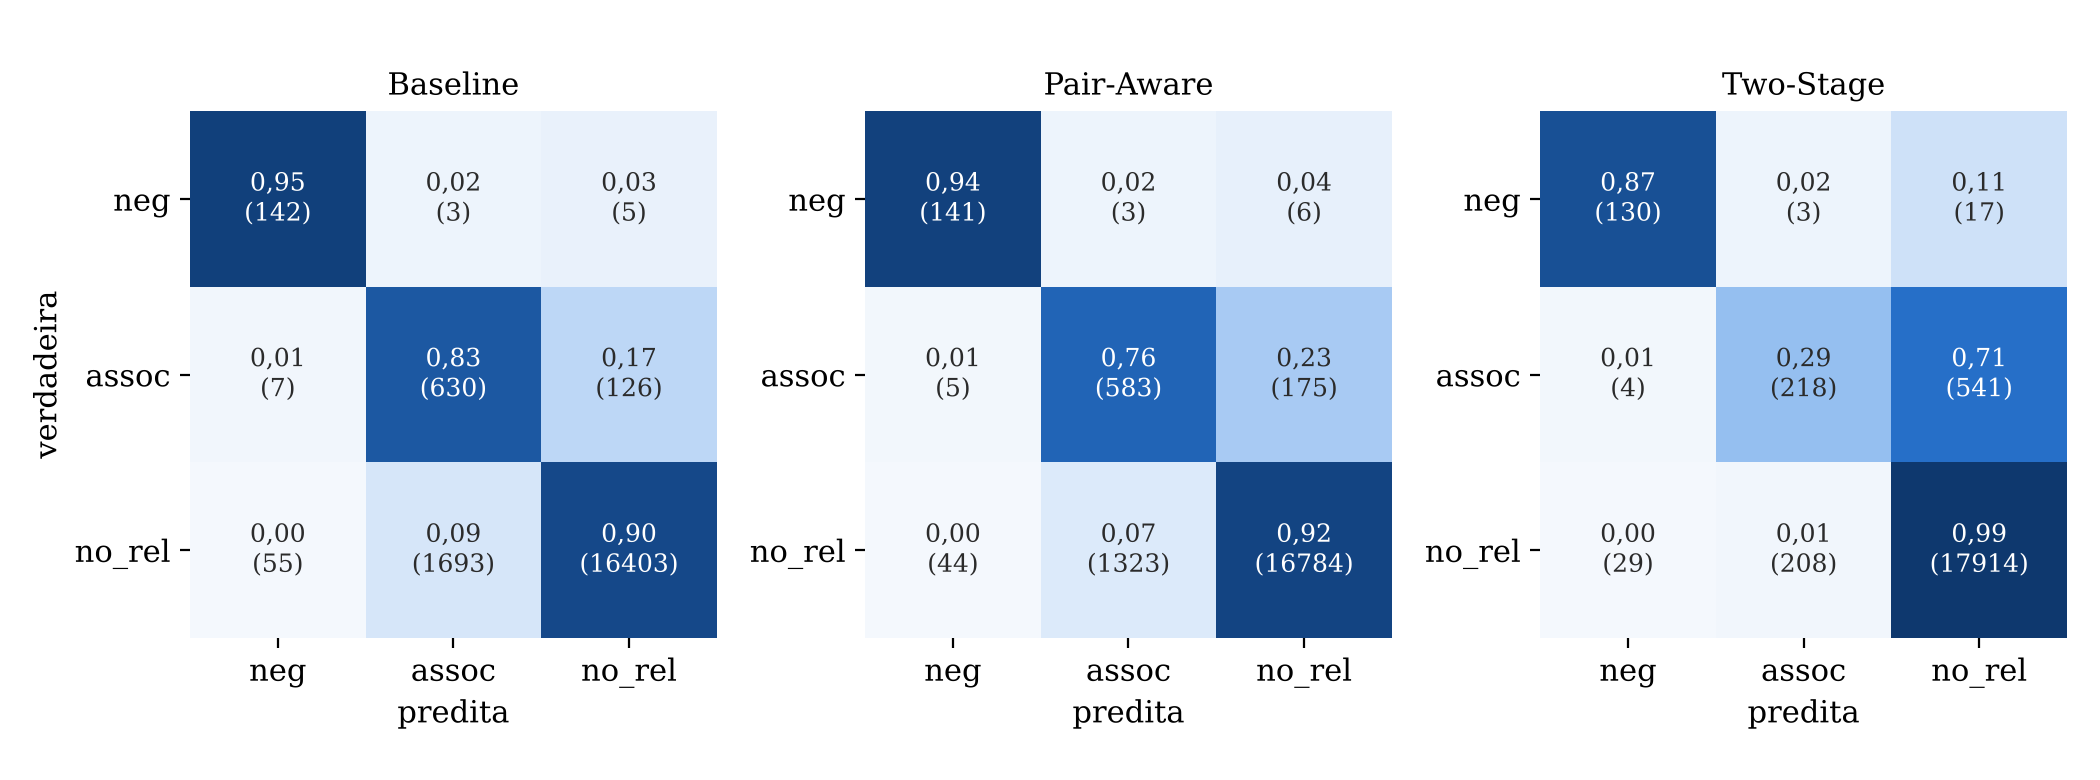
\includegraphics[width=\textwidth]{resultados/matrizes_confusao_dev.png}\\[4pt]
  {\footnotesize Fonte: elaborado pelo autor.}
\end{figure}

\section{O Two-Stage em detalhe}
\label{sec:resultados_twostage}

No estágio 1, a época selecionada pela AP de \texttt{relacao} foi a segunda das três
($0{,}544$), e as épocas executadas em sessão única levaram cerca de uma hora. No estágio 2, medido só sobre os 913
pares do DEV com relação anotada, o F1 de \texttt{negation\_of} ficou entre $0{,}943$
e $0{,}970$ ao longo das dez épocas, a selecionada foi a oitava ($0{,}970$), e cada
época levou cerca de três minutos, por ser treinado só sobre os pares com relação
anotada. A evolução completa por época dos dois estágios está no
Apêndice~\ref{ap:historico}. Esses números descrevem cada estágio isoladamente e não
são resultados da arquitetura, porque o estágio 2 nunca vê, na inferência, os pares
que o estágio 1 não roteia.

A \autoref{fig:tau} mostra o efeito de $\tau$ sobre o
\emph{pipeline} completo (a tabela completa está no Apêndice~\ref{ap:tau}). O F1 de
\texttt{negation\_of} cresce com $\tau$, de $0{,}733$ em $\tau=0{,}05$ até $0{,}8307$
em $\tau=0{,}95$, enquanto o macro-F1 cresce até $0{,}751$ em $\tau=0{,}90$ e cai
para $0{,}725$ em $\tau=0{,}95$. O valor congelado, $0{,}95$, é o extremo superior da
grade e venceu $\tau=0{,}90$ por pouco no critério do protocolo ($0{,}8307$ contra
$0{,}8293$), mas reduziu os pares roteados ao estágio 2 de $1\,303$ para $592$; como
os pares não roteados recebem \texttt{no\_relation}, essa redução se reflete
diretamente na queda do \emph{recall} de \texttt{associated\_with}.

\begin{figure}[htbp]
  \centering
  \caption{Two-Stage no DEV: F1 de \texttt{negation\_of} e macro-F1 do \emph{pipeline} completo em função do limiar $\tau$.}
  \label{fig:tau}
  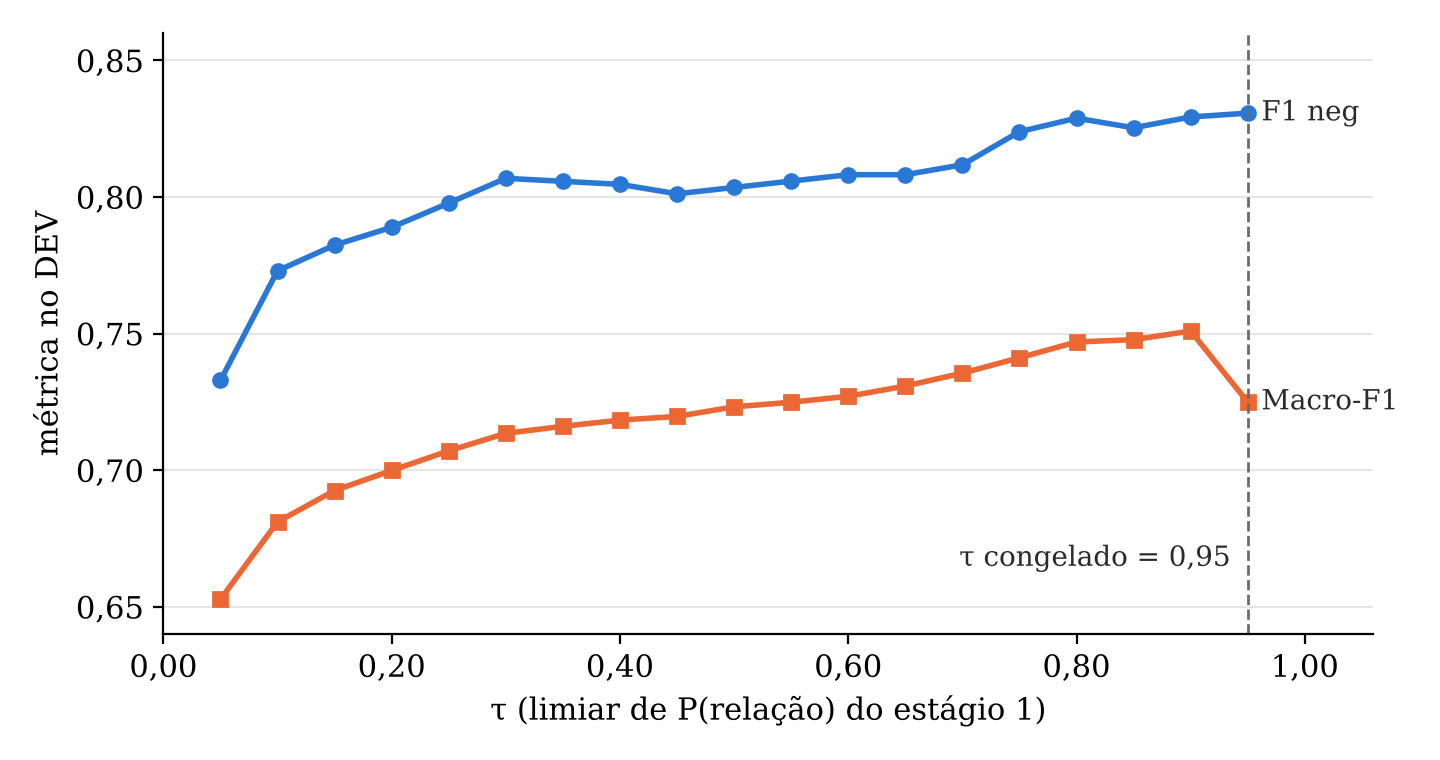
\includegraphics[width=0.85\textwidth]{resultados/tau_two_stage.png}\\[4pt]
  {\footnotesize Fonte: elaborado pelo autor.}
\end{figure}

Com $\tau=0{,}95$, o estágio 1 encaminha ao estágio 2
$592$ pares, dos quais $237$ não têm relação anotada. Ele recupera $88{,}7\%$ dos
pares \texttt{negation\_of}, mas só $38{,}9\%$ do conjunto de pares com relação, e,
entre os pares roteados que têm relação, o estágio 2 acerta o tipo em $98{,}0\%$
dos casos. Nesta execução, portanto, as perdas do Two-Stage concentram-se no estágio 1
e no limiar, e não na distinção entre os tipos.

\section{Comparações pareadas descritivas}
\label{sec:resultados_comparacoes}

A Tabela~\ref{tab:dev_comparacoes} aplica ao DEV, apenas de forma descritiva, os
testes que o protocolo prevê para o teste. No F1 de \texttt{negation\_of}, o
Two-Stage fica à frente de todos os sistemas, mas nenhuma dessas diferenças é
distinguível de zero, nem mesmo contra o baseline calibrado, controle exigido pelo
protocolo para atribuir o efeito à arquitetura; contra a Pair-Aware, a vantagem é de
apenas $+0{,}0013$. A única diferença com IC95\% inteiramente acima de zero é a da
Pair-Aware sobre o baseline ($+0{,}0272$, $[+0{,}0052;\,+0{,}0506]$). Entre
\emph{encoders}, o intervalo é centrado em zero.

%% GERADO por analise/gerar_artefatos_tcc.py -- nao edite a mao.
\begin{table}[htbp]
  \centering
  \caption{Comparações pareadas \textbf{descritivas} no DEV: diferença no F1 de \texttt{negation\_of}, IC95\% e valor-$p$ do \emph{bootstrap} pareado (10.000 reamostras, semente 42) e McNemar exato sobre os acertos globais ($b/c$: só A acerta / só B acerta).}
  \label{tab:dev_comparacoes}
\resizebox{\textwidth}{!}{%
  \begin{tabular}{lrrrrr}
  \toprule
  Comparação (A $-$ B) & $\Delta$F1 neg & IC95\% & $p$ & $b/c$ & $p$ McNemar \\
  \midrule
Two-Stage $-$ Baseline & $+0{,}0284$ & $[-0{,}0079;\,+0{,}0650]$ & 0{,}127 & 1517/430 & $<0{,}001$ \\
Two-Stage $-$ Baseline calibrado & $+0{,}0213$ & $[-0{,}0113;\,+0{,}0543]$ & 0{,}208 & 1512/429 & $<0{,}001$ \\
Baseline calibrado $-$ Baseline & $+0{,}0071$ & $[-0{,}0121;\,+0{,}0260]$ & 0{,}469 & 8/4 & 0{,}388 \\
Two-Stage $-$ Filtro léxico & $+0{,}0125$ & $[-0{,}0187;\,+0{,}0439]$ & 0{,}433 & 1509/430 & $<0{,}001$ \\
Two-Stage $-$ Pair-Aware & $+0{,}0013$ & $[-0{,}0327;\,+0{,}0347]$ & 0{,}963 & 1137/383 & $<0{,}001$ \\
Pair-Aware $-$ Baseline & $+0{,}0272$ & $[+0{,}0052;\,+0{,}0506]$ & 0{,}012 & 588/255 & $<0{,}001$ \\
Two-Stage $-$ Pair-Aware MLP & $+0{,}0135$ & $[-0{,}0223;\,+0{,}0486]$ & 0{,}468 & 1122/380 & $<0{,}001$ \\
BERTimbau-base (baseline) $-$ BioBERTpt-all (baseline) & $-0{,}0023$ & $[-0{,}0295;\,+0{,}0253]$ & 0{,}877 & 499/337 & $<0{,}001$ \\
  \bottomrule
  \end{tabular}}\\[2pt]
  {\footnotesize Descritivas: $\tau$ (Two-Stage) e $t$ (calibrado) foram escolhidos neste DEV, e a época de cada modelo também; não substituem as comparações pré-registradas no TEST.}\\[4pt]
  {\footnotesize Fonte: elaborado pelo autor.}
\end{table}


O McNemar rejeita a igualdade em quase todas as comparações, mas responde a outra
pergunta: ele incide sobre o acerto global, dominado pela classe
\texttt{no\_relation}. O Two-Stage, por exemplo, acerta muito mais pares no total
(acurácia de $0{,}958$, contra $0{,}901$ do baseline), em grande parte porque prevê
\texttt{no\_relation} com mais frequência, o que não se traduz em vantagem na
classe-alvo nem no macro-F1. A única comparação sem diferença no McNemar é a do
baseline calibrado com o baseline, cujas predições diferem em apenas 12 pares.

\section{Resultado exploratório}
\label{sec:resultados_exploratorios}

A variante Pair-Aware MLP, fora do protocolo, foi treinada com a mesma entrada, os
mesmos dados e a mesma seleção da Pair-Aware do protocolo, mudando apenas a cabeça.
Ela teve \emph{recall} de \texttt{negation\_of} um pouco maior ($0{,}953$) e precisão
menor ($0{,}715$), e terminou com F1 de $0{,}817$ e macro-F1 de $0{,}737$, ambos abaixo
da Pair-Aware linear; a diferença para o Two-Stage no F1 de \texttt{negation\_of}
também não é distinguível de zero (Tabela~\ref{tab:dev_comparacoes}). Os valores
completos estão no Apêndice~\ref{ap:exploratoria}. Por ser exploratório, esse
resultado não é evidência confirmatória e não entra na escolha da estratégia de
referência.
